\documentclass{article}


\usepackage[utf8]{inputenc}
\usepackage[english]{babel}
\usepackage{authblk,url}
\usepackage{amssymb,amsmath,amsthm,twoopt,xargs,mathtools}
\usepackage{times,ifthen}
\usepackage{fancyhdr,xcolor}

\title{}
\date{}

%\author[$\wr$]{Mathis Chagneux}
\author[$\dag$]{XXX}
%\affil[$\wr$]{{\small LTCI, T\'el\'ecom Paris, Institut Polytechnique de Paris, Palaiseau.}}

\affil[$\dag$]{{\small CMAP, \'Ecole Polytechnique, Institut Polytechnique de Paris, Palaiseau.}}

\lhead{}
\rhead{}

\DeclareUnicodeCharacter{2212}{-}
\usepackage{geometry}
\pagestyle{fancy}

\def\dimX{d}
\def\dimY{m}
%\def\Xset{\mathsf{X}}
\def\Xset{\mathbb{R}^d}
\def\Yset{\mathsf{Y}}
\newcommand{\mk}{\kernel{G}}
\newcommand{\hk}{\kernel{Q}}
\newcommand{\md}[1]{g_{#1}}
\newcommand{\SmoothFigSize}{0.27}

\newcommand{\logllh}[1]{\ell_{#1}}
\newcommand{\llh}[1]{\mathsf{L}_{#1}}
\newcommand{\testf}{\mathsf{h}}

\newcommandx\filtderiv[2][1=]{
\ifthenelse{\equal{#1}{}}
	{\eta_{#2}}
	{\eta_{#2}^\N}
}
\newcommand{\pred}[1]{\pi_{#1}}
\newcommand{\parvec}{\theta}
\newcommand{\parspace}{\Theta}
\newcommand{\tstatletter}{\kernel{T}}
\newcommand{\retrok}{\kernel{D}}
\newcommandx\tstat[2][1=]{
\ifthenelse{\equal{#1}{}}
	{\tstatletter_{#2}}
	{\tau_{#2}^{#1}}
}
\newcommandx\tstathat[2][1=]{
\ifthenelse{\equal{#1}{}}
	{\tstatletter_{#2}}
	{\widehat{\tau}_{#2}^{#1}}
}
\newcommand{\af}[1]{h_{#1}}
\newcommand{\deriv}{\nabla_{\parvec}}

\newcommand{\kernel}[1]{\mathbf{#1}}
\newcommand{\bmf}[1]{\set{F}(#1)}
\newcommand{\set}[1]{\mathsf{#1}}

\newcommandx{\bk}[2][1=]{
\ifthenelse{\equal{#1}{}}
{\overleftarrow{\kernel{Q}}_{#2}}
{\overleftarrow{\kernel{Q}}_{#2}^{#1}}
}

\newcommandx{\bkhat}[2][1=]{
\ifthenelse{\equal{#1}{}}
{\widehat{\kernel{Q}}_{#2}}
{\widehat{\kernel{Q}}_{#2}^{#1}}
}

\newcommand{\lk}{\kernel{L}}
\newcommand{\idop}{\operatorname{id}}
\newcommand{\hd}[1]{q_{#1}}
\newcommand{\hdhat}[1]{\widehat{q}_{#1}}


\newcommand{\addf}[1]{\termletter_{#1}}
\newcommand{\addfc}[1]{\underline{\termletter}_{#1}}
\newcommand{\adds}[1]{\af{#1}}
\newcommand{\term}[1]{\termletter_{#1}}
\newcommand{\termletter}{\tilde{h}}
\newcommand{\N}{N}
\newcommand{\partpred}[1]{\pi_{#1}^\N}
\newcommand{\tstattil}[2]{\tilde{\tau}_{#2}^{#1}}
\newcommandx{\K}[1][1=]{
\ifthenelse{\equal{#1}{}}{{\kletter}}{{\widetilde{\N}^{#1}}}}
\newcommand{\hkup}{\bar{\varepsilon}}
\newcommand{\bi}[3]{J_{#1}^{(#2, #3)}}
\newcommand{\bihat}[3]{\widehat{J}_{#1}^{(#2, #3)}}

\newcommand{\kletter}{\widetilde{\N}}

\def\sigmaX{\mathcal{X}}
\def\sigmaY{\mathcal{Y}}
\def\1{\mathds{1}}
\def\pE{\mathbb{E}}
\def\pP{\mathbb{P}}
\def\plim{\overset{\pP}{\longrightarrow}}
\def\dlim{\Longrightarrow}
\def\gauss{\mathcal{N}}


\newcommand{\esssup}[2][]
{\ifthenelse{\equal{#1}{}}{\left\| #2 \right\|_\infty}{\left\| #2 \right\|^2_{\infty}}}


\newcommand{\swght}[2]{\ensuremath{\omega_{#1}^{#2}}}

\newtheorem{assumptionA}{\textbf{A}\hspace{-3pt}}
\newcommand{\rset}{\ensuremath{\mathbb{R}}}
\newcommand{\iid}{i.i.d.}

\newcommand{\smwght}[3]{\tilde{\omega}_{#1|#2}^{#3}}
\newcommand{\smwghtfunc}[2]{\tilde{\omega}_{#1|#2}}

\newcommand{\smpart}[3]{\ensuremath{\tilde{\xi}_{#1|#2}^{#3}}}
\def\aux{{\scriptstyle{\mathrm{aux}}}}
\newcommand{\bdm}{\mathsf{TwoFilt}_{bdm}}
\newcommand{\fwt}{\mathsf{TwoFilt}_{fwt}}

\newcommand{\kiss}[3][]
{\ifthenelse{\equal{#1}{}}{r_{#2|#3}}
{\ifthenelse{\equal{#1}{fully}}{r^{\star}_{#2|#3}}
{\ifthenelse{\equal{#1}{smooth}}{\tilde{r}_{#2|#3}}{\mathrm{erreur}}}}}

\newcommand{\chunk}[4][]%
{\ifthenelse{\equal{#1}{}}{\ensuremath{{#2}_{#3:#4}}}{\ensuremath{#2^#1}_{#3:#4}}
}

\newcommand{\kissforward}[3][]
{\ifthenelse{\equal{#1}{}}{p_{#2}}
{\ifthenelse{\equal{#1}{fully}}{p^{\star}_{#2}}
{\ifthenelse{\equal{#1}{smooth}}{\tilde{r}_{#2}}{\mathrm{erreur}}}}}

\newcommand{\instrpostaux}[1]{\ensuremath{\upsilon_{#1}}}
\newcommandx\post[2][1=]{
\ifthenelse{\equal{#1}{}}
	{\phi_{#2}}
	{\phi_{#2}^\N}
}

\newcommandx\posthat[2][1=]{
\ifthenelse{\equal{#1}{}}
	{\widehat{\phi}_{#2}}
	{\widehat{\phi}_{#2}^\N}
}

\newcommand{\adjfunc}[4][]
{\ifthenelse{\equal{#1}{}}{\ifthenelse{\equal{#4}{}}{\vartheta_{#2|#3}}{\vartheta_{#2|#3}(#4)}}
{\ifthenelse{\equal{#1}{smooth}}{\ifthenelse{\equal{#4}{}}{\tilde{\vartheta}_{#2|#3}}{\tilde{\vartheta}_{#2|#3}(#4)}}
{\ifthenelse{\equal{#1}{fully}}{\ifthenelse{\equal{#4}{}}{\vartheta^\star_{#2|#3}}{\vartheta^\star_{#2|#3}(#4)}}{\mathrm{erreur}}}}}

\newcommand{\XinitIS}[2][]
{\ifthenelse{\equal{#1}{}}{\ensuremath{\rho_{#2}}}{\ensuremath{\check{\rho}_{#2}}}}
\newcommand{\adjfuncforward}[1]{\vartheta_{#1}}
\newcommand{\rmd}{\ensuremath{\mathrm{d}}}
\newcommand{\eqdef}{\ensuremath{:=}}
\newcommand{\eqsp}{\;}
\newcommand{\ewght}[2]{\ensuremath{\omega_{#1}^{#2}}}
\newcommand{\ewghthat}[2]{\ensuremath{\widehat{\omega}_{#1}^{#2}}}
\newcommand{\epart}[2]{\ensuremath{\xi_{#1}^{#2}}}
\newcommand{\filt}[2][]%
{%
\ifthenelse{\equal{#1}{}}{\ensuremath{\phi_{#2}}}{\ensuremath{\phi_{#1,#2}}}%
}
\newcommand{\Xinit}{\ensuremath{\chi}}
\newcommand{\sumwght}[2][]{%
\ifthenelse{\equal{#1}{}}{\ensuremath{\Omega_{#2}}}{\ensuremath{\Omega_{#2}^{(#1)}}}}
\newcommand{\sumwghthat}[2][]{%
\ifthenelse{\equal{#1}{}}{\ensuremath{\widehat{\Omega}_{#2}}}{\ensuremath{\widehat{\Omega}_{#2}^{(#1)}}}}

\newcounter{hypH}
\newenvironment{hypH}{\refstepcounter{hypH}\begin{itemize}
\item[{\bf H\arabic{hypH}}]}{\end{itemize}}

\newcommand{\marginalset}{\mathsf{U}}

\newcommand{\calF}[2]{\mathcal{F}_{#1}^{#2}}
\newcommand{\calG}[2]{\mathcal{G}_{#1}^{#2}}
\newcommand{\Uset}{\mathsf{U}}
\newcommand{\tcalF}[2]{\widetilde{\mathcal{F}}_{#1}^{#2}}
\newcommand{\tcalG}[2]{\widetilde{\mathcal{G}}_{#1}^{#2}}

\newcommand{\kernelmarg}{\mathbf{R}}

\newcommand{\pplim}{\overset{\pP}{ \underset{\N \to \infty}{\longrightarrow}}}
\newcommand{\ddlim}{\overset{\mathcal{D}}{ \underset{\N \to \infty}{\longrightarrow}}}
\newcommand{\aslim}{\overset{\pP\mathrm{-a.s.}}{ \underset{\N \to \infty}{\longrightarrow}}}

\newcommand{\qg}[1]{\ell_{#1}}
\newcommand{\hatqg}[1]{\mathsf{\ell}_{#1}}

\newcommand{\sfd}{\mathsf{d}}
\newcommand{\X}{\mathbf{X}}
\newcommand{\x}{\mathbf{x}}
\newcommand{\y}{\mathbf{y}}
\newcommand{\E}{\mathbf{E}}
\newcommand{\e}{\text{e}}
\newcommand{\W}{\mathbf{W}}
\newcommand{\Z}{\mathbf{Z}}
\newcommand{\frob}{:}
\newcommand{\rme}{\mathrm{e}}
\newcommand{\vois}{\mathcal{V}}

\begin{document}

\maketitle

\begin{abstract}

\end{abstract}

\section{Introduction}
\section{Related works}
\section{Bridge sampling quantizers}
 Let $X = (X^1,\ldots,X^n)$ be the observations in $\rset^D$.  It is assumed that the distribution of $X$ depends on a hidden sequence of discrete states taking values in $\{1,\ldots,K\}$ through  embedding vectors $(\rme^1,\ldots,\rme^K)$ in $\rset^m$. In  \cite{oord2017neural}, the authors proposed the Vector Quantised Variational AutoEncoder (VQ-VAE) in which  the encoder network outputs discrete states written $Z_q$ using a continuous endoding vector $Z_e$ mapped onto the nearest element in $(\rme^1,\ldots,\rme^K)$. This approach  does not suffer from usual posterior collapse in VAE setting but invovles many practical tricks and still suffer from serious limitations, see \cite{}.

In this paper, we introduce a diffusion-based generative VQ-VAE. This model allows to propose a VAE approach with an efficient joint training of the prior and the variational approximation. Diffusion-based generative models have recently shown striking results in image generation and can be used in our setting to define a noising/denoising process in a continuous state space to sample sequences of discrete representations. Consider the following model.
$$
p_{\theta}(Z_q^{0:T},U_q^{0:T}, X) %&= p_{\theta,T}(Z_q^T,U_q^T) \left\{\prod_{t=0}^{T-1}p_{\theta,t}(Z_q^t,U_q^t|Z_q^{t+1},U_q^{t+1})\right\}  p_{\theta,0}(X|Z^{0:T}_q,U_q^{0:T})\,,\\
= p^u_{\theta,T}(U_q^T) p^z_{\theta,T}(Z_q^T|U_q^T)\left\{\prod_{t=0}^{T-1}p^u_{\theta,t}(U_q^t|U_q^{t+1})p^z_{\theta,t}(Z_q^t|U_q^t)\right\}p^x_{\theta,0}(X|Z^{0}_q)\,.
$$
In this setting, $\{U_q^t\}_{T\leqslant t\leqslant 0}$ is a continuous latent state and conditionally on $\{U_q^t\}_{T\leqslant t\leqslant 0}$ the $\{Z_q^t\}_{T\leqslant t\leqslant 0}$ are independent with discrete distribution with support $(\rme^1,\ldots,\rme^K)$.  The prior distribution of  $U_q^T$ is assumed to be uninformative and this is the sequence of denoising transition densities $\{p^u_{\theta,t}\}_{0\leqslant t\leqslant T-1}$ which provides the final latent state $Z_q^0$ which is used in the decoder, i.e. the conditional law of $X$ given the latent states.
Most approaches \cite{} using diffusion probabilistic models for $\{U_q^t\}_{T\leqslant t\leqslant 0}$ are based on a fixed diffusion process. A notable exception is \cite{} where the authors learned a Gaussian diffusion process. This specific choice was motivated by the design of the generative model which required to "invert" the diffusion process, i.e. to sample from a bridge process associated with Stochastic Differential Equation (SDE), which is explicit only for very few classes of diffusions.

As the conditional law $p_{\theta}(Z_q^{0:T},U_q^{0:T}| X)$ is not available explicitly, this work focuses on  variational approaches to provide an approaximation. Consider first an encoding function $f_\eta$ and write $Z_\rme= f_\eta(X)$. Then, consider the following variational familly:
$$
q_{\varphi}(Z_q^{0:T},U_q^{0:T}| X) = q^u_{\varphi,0}(U_q^0 | Z_\rme)q_{\varphi,0}^z(Z_q^0|U_q^0) \prod_{t=1}^T\left\{ q^t_{\varphi,t}(U_q^t|U_q^{t-1})q^z_{\varphi,t}(Z_q^t|U_q^t)\right\}\,.
$$
Using the auxiliary variational inference framework (AVI) and following \cite{}, define the loss function:
\begin{multline*}
\mathcal{L}(\theta, \varphi) = \mathbb{E}_{q_\varphi} \left[ \log p_\theta(U_q^{0},Z_q^{0}|U_q^{0},Z_q^{0})\right]\\
 - \sum_{t=1}^{T}\mathbb{E}_{q_\varphi} \left[\mathrm{KL}(q_\varphi(Z_q^{t-1},U_q^{t-1}|Z_q^t,U_q^{t},Z_q^0,U_q^{0})\|p_\theta(Z_q^{t-1},U_q^{t-1}|Z_q^t,U_q^t)) \right]\,.
\end{multline*}
In our case, this loss reduces to
$$
\mathcal{L}(\theta, \varphi) = \mathbb{E}_{q_\varphi} \left[ \log p_\theta(U_q^{0},Z_q^{0}|U_q^{0},Z_q^{0}) - \sum_{t=1}^{T}\mathrm{KL}(q^u_{\varphi,t}(U_q^{t-1}|U_q^{t},U_q^{0})\|p^u_{\theta,t}(U_q^{t-1}|U_q^t)) \right]\,.
$$
Bridge sampling quantizers then proceed as follows.
\begin{enumerate}
\item Define the noising transition density $q^u_{\varphi,t}(U_q^{t}|U_q^{t-1})$ as the transition density of a SDE.
\item Compute the bridge sampler $q^u_{\varphi,t}(U_q^{t-1}|U_q^{t},U_q^{0})$ or approximate it using Monte Carlo simulation and/or discretization schemes.
\item Define $p^u_{\theta,t}(U_q^{t-1}|U_q^t)$ as $q_\varphi(U_q^{t-1}|U_q^{t},U_q^{0})_{|U_q^{0} = g_{\theta,t}(U_q^t)}$ where $g_{\theta,t}$ is a deep neural network (see below) provides a denoised latent state from $U_q^t$.
\end{enumerate}
\section{Denoiser based on bridge sampling}

\subsection{Application to Langevin diffusions}
Let $\pi$ be a probability distribution function with respect to the Lebesgue measure such that $\pi \propto \mathrm{exp}(-G)$ where $G$ is continuously differentiable.
We consider a sampling method based on the Euler discretization of the overdamped Langevin
stochastic differential equation (SDE):
$$
\mathrm{d}U_t = -\nabla G(U_t)\mathrm{d}t + \sqrt{2}\mathrm{d}W_t\,.
$$
Under standard assumptions, see \cite{}, the convergence to $\pi$ holds at geometric rate. In this case, $\pi$ is the equilibrium distribution, and our model will target this distribution as initial law of $U_q^T$

\subsection{Application to Ornstein-Uhlenbeck bridges}
\paragraph{Adding noise. }
In the previous example the noising and denoising problem over the random variables $\{U_q^t\}_{0\leqslant t\leqslant T}$ is sensitive to the initial scaling of the distance between embedded data and codebooks. An appealing solution to avoid this problem is to normalize all the distances and use for instance spherical projection. Then, then the $q_\varphi$ may  be defined as sampling for the solution of a Stochastic Differential Equation (SDE) to add noise to the  normalized inputs. Consider for instance
$$
\mathrm{d}U_t = -\theta (U_t - U_*)\mathrm{d}t + \sigma\mathrm{d}W_t
$$
where $U_*$ is the target state at the end of the noising process (can be chosen as 0 for the initial simulation) and $W_t$ is a standard Browian motion. We can define $q_\varphi$ by integrating this SDE along small step-sizes. In this setting, $q_\varphi(U_q^{t}|U_q^{t-1})$ is a Gaussian probability density function with mean $U_* + (U_q^{t-1}-U_*)\mathrm{e}^{-\theta \delta}$ and variance $\sigma^2(1-\mathrm{e}^{-2\theta\delta})/(2\theta)$ where $\delta>0$ is the step-size between $t-1$ and $t$. Asymptotically the process is a Gaussian with mean $U_*$ and variance $1/(2\theta)$ which means that the samples will fluctuate around $U_*$.

\paragraph{Bridge to denoise. }
The denoising process amounts then to sampling from the bridge associated with the SDE, i.e. sampling $U_q^s$ given $U_q^0$ and $U_q^t$ where $0<s<t$. The law of this Bridge is explicit for the Brownian diffusion and the Ornstein-Uhlenbeck diffusion. Write for all $s>0$, $v_s = \sigma^2(1-\mathrm{e}^{-2\theta\delta s})/(2\theta)$.
Following the same steps as in the previous section,
$$
q^u_{\varphi,t}(U_q^{t-1}|U_q^{t},U_q^{0}) \propto q^u_{\varphi,t}(U_q^{t-1}|U_q^{0}) q^u_{\varphi,t}(U_q^{t}|U_q^{t-1})
$$
so that $q^u_{\varphi,t}(U_q^{t-1}|U_q^{t},U_q^{0})$ is a Gaussian probability density function with mean
$$
\tilde \mu_{t|t-1,0} = \frac{\sigma^2_{t|t-1,0}}{v_{t-1}}\left(U_q^0\mathrm{e}^{-\theta\delta(t-1)} +U_*(1-\mathrm{e}^{-\theta\delta(t-1)})\right) + \frac{\sigma^2_{t|t-1,0}}{v_{1}}\mathrm{e}^{-\theta\delta}\left(U_q^t - U_*(1 - \mathrm{e}^{-\theta\delta} )\right)
$$
and variance
$$
\tilde \sigma^2_{t|t-1,0} = \left(\frac{1}{v_{t-1}} + \frac{\mathrm{e}^{-2\theta\delta}}{v_1}\right)^{-1}\,.
$$
 Therefore, $p^u_{\theta,t}(U_q^{t-1}|U_q^t)$ can be parameterized similarly by replacing $U_q^0$ by a deep neural networks based regressor.

\paragraph{Similarities with the "Ho diffusion". }
Consider a simplified Ornstein-Uhlenbeck diffusion ($U_* = 0$, $\theta = 1$),
$$
\mathrm{d}U_t = -U_t\mathrm{d}t + \sqrt{2}\mathrm{d}W_t\,.
$$
 In this setting, $q^u_{\varphi,t}(U_q^{t}|U_q^{t-1})$ is a Gaussian probability density function with mean $U_q^{t-1}\mathrm{e}^{-\delta}$ and variance $(1-\mathrm{e}^{-2\delta})$ where $\delta>0$ is the step-size between $t-1$ and $t$. This is exactly the noise process proposed by Ho et al. with $\sigma^2_t = 1 - \mathrm{e}^{-2\delta}$. It is enough to choose a step-size $\delta$ depending on  $t$ to recover exactly their noise process.

\subsection{Application to other bridges}

\subsection{Experiments on toy problems}

Consider a dataset of $N$ discrete vectors: $X \in {1,...K}^d$ where K is an integer (i.e. size of a codebook or vocabulary) and $d$ the dimension of the vector. The dimensions of the vector are not independant (i.e. integer pixel values in a picture).

A discrete diffusion process such as [Welling] would slowly add noise in the discrete vectors, by replacing a random coordinate of the vector by a uniform integer [Welling] or a mask [Microsoft, Structured denoising diffusion models in discrete state-spaces].

We propose instead to associate with each of the $K$ code an embedding $\{e_k\}_{1 \leq k \leq K}$ continuous vector of dimension $m$ and normalized: $e_k$ is on the unit sphere. This embedding projection is random. We denote $E(X) \in \rset^{d \times m}$ the continuous embedding projection of vector $X$

In this setting, we apply a simple diffusion bridge as described previously, with $U_0 = E(X)$:
$$
\mathrm{d}U_t = -\theta U_t \mathrm{d}t + \sigma\mathrm{d}W_t
$$

\paragraph{Methods to compare} We compare the discrete generative process induced by the reverse diffusion process with the following methods:

\begin{itemize}
	\item \textbf{Continuous diffusion}: Ours (with varying $\theta$ (and bridges?)) ; On logits (defined further) [Ho ?]
	\item \textbf{Discrete diffusion}: [Welling] and [Structured denoising diffusion models in discrete state-spaces, Microsoft]
	\item Autoregressive method modeling $X$ as a sequence of $d$ integers
\end{itemize}

\paragraph{Settings} We will consider the two settings:

\begin{itemize}
	\item Our data points are discrete vectors, embedded on the sphere.\footnote{in the case of a continuous diffusion, logits are the one-hot encoding of the discrete values.}
	\item For each datapoint, we add a noise over the vector embeddings, accounting for a distribution over the closest embeddings. This second setting allows to model points that are distribution over discrete values rather than a single discrete value, by considering the distance / similarity between the continuous vector and the codebook embeddings.\footnote{in the case of a continuous diffusion, logits are the distances between the vector $X$ and the codebooks $e_k$.}
\end{itemize}

\paragraph{Evaluation} We study the dynamics of the noising and denoising process, and compare the efficiency of the methods through:
\begin{itemize}
	\item reconstruction error (crossentropy) (Start with dataset sample $U_0$, run noising bridge to get $U_T$, then denoising yielding $\hat U_0$. Compare $\hat U_0$ with original $U_0$.)
	\item diversity when sampling:
		\begin{itemize}
			\item Sample multiple $U_T$ from the uniform/gaussian distribution with mean $0_m$, run the denoising bridge for each, compare diversity of resulting vectors ;
			\item Sample a single point from the uniform/gaussian distribution with mean $0_m$, run multiple denoising bridge, compare diversity;
		\end{itemize}
	\item efficiency when sampling
	\item Distribution compared to original dataset (KL to uniform, histogram of specific pixels)
	\item Sanity check:
		\begin{itemize}
			\item Check that step size during denoising remains small ;
			\item Check that estimation $\tilde U_0$ is \textit{regular} when $t : T \rightarrow 0$.
		\end{itemize}
\end{itemize}

\paragraph{Dataset} We could use the following toy datasets:

\begin{itemize}
	\item a complete toy dataset (size $N=1000$, $K=10$, $d=10$, $m=2$), with a simple dependency between dimensions of $X$, for instance $X^0$ uniform, and $X^{i+1} = X^i \pm 1 \mod K$
	\item a small text dataset with characters (size $N=1000$, vocabulary $K=27$, fixed sequence length $d=10$, $m=2$)
	\item a small discretized and downsampled version of MNIST (size $N=1000$, vocabulary $K=8$, fixed sequence length $d=8 \time 8$, $m=2$)
\end{itemize}

\subsection{Experiments with a VQ-VAE}



\bibliographystyle{apalike}
\bibliography{vqvae}



\clearpage
\newpage

\section{First Experiments}
First experiments were focused on baselines on images and a few timeseries. \footnote{List of experiments \& datasets to validate the new approach and compare to vq-vae \url{https://docs.google.com/document/d/1a7lhplsBraTD3qmvsHXdoPmQj00YijT2XMWpHEFeb58/edit}}

\begin{itemize}
	\item \textbf{Datasets} implemented: {\em MNIST}, {\em FashionMNIST}, {\em Cifar-10}, and timeseries {\em Weather} and {\em Air quality}.
	\item \textbf{Baselines and architectures} Simple VAE model, with Feed Forward, Convolutional (simple) and ResNet encoder / Decoder; IWAE ; VQ-VAE, with standard implementation (straight-through gradient passing over the codebook), including the exponential moving average trick to stabilize the training of the codebook.

	A pixelCNN (pixelSnail) autoregressive \textit{prior} model, to learn the unconditionnal marginalized $q(z_q)$ by encoding the full dataset using the encoder.

	VQ-VAE with Gumbel-softmax trick, which alleviates the need for other gradient copying tricks and unstabilities (very used in VQ-VAE implementations)

	The Sequential mixture VQ-VAE, as described below.
  \item \textbf{Metrics} implemented: NLL on valset, Bits per dim ; FID score (pictures only) ; Inception Score (pictures only, in progress).
\end{itemize}

The sequential mixture VAE has only been tested on image generation for now. In first experiments, it achieves slightly worse scores than the standard VQ-VAE on FashionMNIST (the NLL of seqVQVAE is $0.1$ worse than VQ-VAE). The following figures show the first reconstructions. However, we did not tune the hyperparameters or the model heavily, as the sequential model does not naturally fit very well the image generation problem (it would be better on sequential data).

\begin{figure}[htp]
    \begin{center}
    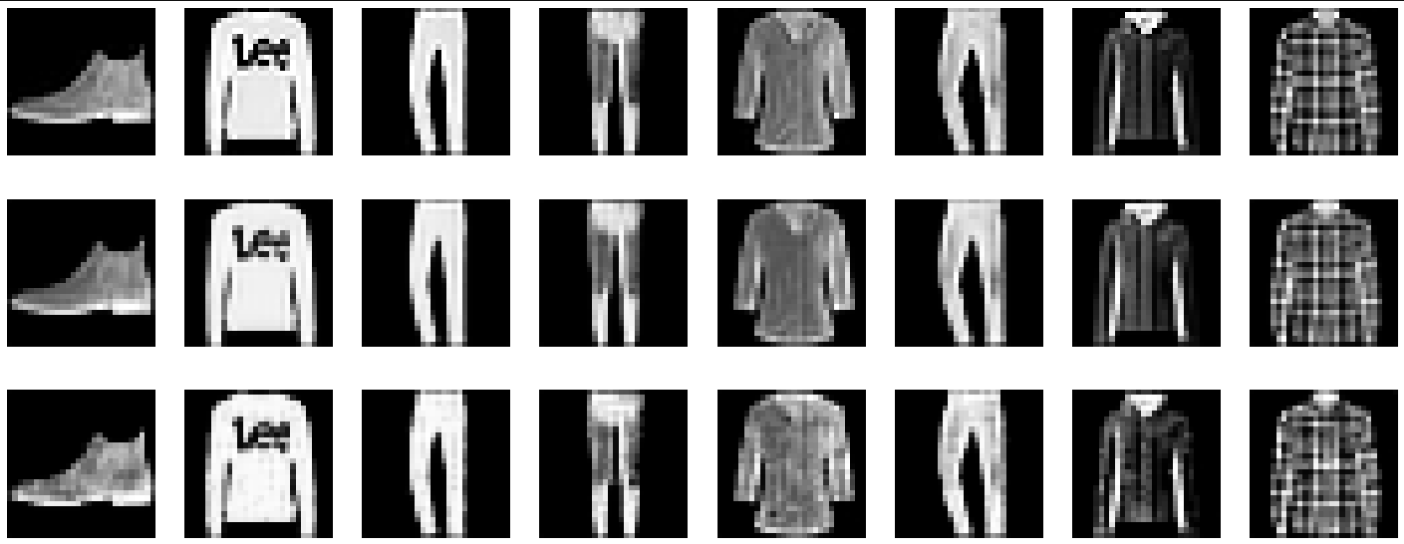
\includegraphics[width=0.37\textwidth]{images/seqvae3.png}
    \caption{FashionMNIST first reconstruction experiments. Top to bottom: originals, Reconstructions of VQ-VAE, Reconstructions of SeqVAE}
    \end{center}
\end{figure}

\begin{figure}[htp]
    \begin{center}
    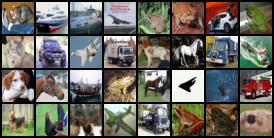
\includegraphics[width=0.37\textwidth]{images/originals.png} \\
		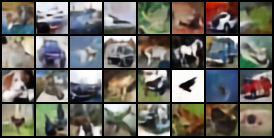
\includegraphics[width=0.37\textwidth]{images/vqvae2.png} \\
		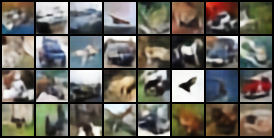
\includegraphics[width=0.37\textwidth]{images/seqvqvae2.png}
    \caption{Cifar first reconstruction experiments. Top to bottom: originals, Reconstructions of VQ-VAE, Reconstructions of SeqVAE}
    \end{center}
\end{figure}


\clearpage
\newpage

\section{RNN-based mixture vq-vae with "posterior" training of the prior (for time series)}
 Let $(X^1,\ldots,X^n)$ be the observations in $\rset^D$.  It is assumed that the distribution of $X$ depends on a hidden sequence of discrete states $(z_q^1,\ldots, z_q^n)$ taking values in $\{1,\ldots,K\}$ through  embedding vectors $(\rme^1,\ldots,\rme^K)$ in $\rset^m$.

\paragraph{Decoder i.e. generative model - mixture vq-vae.}
Following the standard vq-vae approach, during training it is assumed that the prior distribution of the hidden states is uniform on $\{1 \cdots K\}$. %$p_\theta(z_q)$ is uniform (i.e. we do not estimate the prior during this training phase).
%$$
%p_\theta(z_q) = \prod_{j=1}^m p(z_q^j)\eqsp,
%$$
%where $p$ is the uniform distribution on $\{1 \cdots K\}$.
Then, consider the following model:
$$
p_{\theta}(X|z_q) = \prod_{j=1}^n p_{\theta}(X^j|\vois(z_q^j)) = \varphi_{\mu_\theta(\bar e^j),\Sigma_\theta(\bar e^j)}(X)\eqsp,
$$
where $\vois(z_q^j)$ are the vectors in a neighborhood of  $z_q^j$, $\bar e^j = \{e^{z_q^\ell}\;;\; z_q^\ell\in \vois(z_q^j)\}$ and where $\varphi_{\mu,\sigma}$ is the Gaussian probability density function with mean $\mu$ and variance matrix $\Sigma$. We may consider for instance $\vois(z_q^j) = \{z_q^{j-p} \cdots z_q^j\}$, a neighborhood given by a one dimensional convolution.

\paragraph{Encoder - mixture vq-vae.} Consider an encoding function $f_\theta$ and write
$$
(z_\rme^1,\ldots, z_\rme^m) = f_\eta(X^{1:n})\eqsp.
$$
Note that the function $f_\eta$ does not build as many encoding states $(z_\rme^1,\ldots, z_\rme^m)$ as the number of observations.
%The parameters $\theta$ are estimated through gradient descent during the training.

\paragraph{Quantization} Consider a variational family $q_\varphi(z_q^{1:m}|z_e^{1:m})$ given by a recurrent neural network. Set $h^0 = 0$, and for all $1 \leq j \leq m$ and all $1 \leq k \leq K$,
\begin{align*}
    h^j &= \tanh(W_z z_e^j + W_h h^{j-1} + b)\,, \\
    p^j &= \texttt{softmax}\left(\left\{- \| \rme_k - h^j\|^2\right\}_{1\leqslant k \leqslant K}\right)\,,
\end{align*}
where $W_z, W_h$ and $b$ are the unknownweight matrices and vector of the neural network.
%In the specific conditions where $W_z = I_d$ and $W_h = b = 0$, these equations lead to
%$$
%p^j_k = \texttt{softmax}(- \| \rme_k - \tanh(z_e^j) \|^2)\,.
%$$
Codebook vectors are sampled  from the categorical distribution based on the computed $p^j_{1:K}$:
$$
q_\varphi(z_q^{1:m} | z_e^{1:m}) = \prod_{j=1}^m p_\theta(z_q^j|z_e^{1:j}) = \prod_{j=1}^m \texttt{Cat}(\{p^j_k\}_{k=1}^K)\,.
$$
During training, we replace the categorical distribution by a Gumbel distribution, in order to define a differentiable quantization.

\paragraph{Training}
We minimize the loss
$$
\mathcal{L}(\theta, \varphi) = \mathbb{E}_{q_\varphi} \left[ \log\left(\frac{p_\theta(x|z_q)}{q_\varphi(z_q|z_e)}\right) \right]
$$
If we consider $\Sigma_\theta$ to be a diagonal matrix, with values $\Sigma_\theta = \texttt{diag}(\{\sigma_{\theta, i}^2\}_{i=1}^d)$:
\begin{align*}
    \log p_\theta(x|z_q^j) &= \log \varphi_{\mu_\theta(\vois(z_q^j)),\Sigma_\theta(\vois(z_q^j))}(x) \\
			   &= \log\left(|\Sigma_\theta(\vois(z_q^j))|^{-\frac{1}{2}} \exp\left(-\frac{1}{2}(x - \mu_\theta(\vois(z_q^j)))^T \Sigma_\theta(\vois(z_q^j))^{-1} (x - \mu_\theta(\vois(z_q^j))) \right)\right) \\
			   &= -\sum_{i=1}^d \log(\sigma_{\theta, i}(\vois(z_q^j))) -\frac{1}{2} \sum_{i=1}^d \frac{(x_i - \mu_\theta(\vois(z_q^j)))^2}{\sigma_{\theta, i}^2(\vois(z_q^j))}
\end{align*}
where constant terms have been omitted.

\paragraph{Sequential data case}
In the case of sequential data, we may consider the model
$$
p_{\theta}(X|z_q) = \prod_{j=1}^n p_{\theta}(X^j|\vois(z_q^j)) = \varphi_{\mu_\theta(\bar e^j),\Sigma_\theta(\bar e^j)}(X)\eqsp,
$$
Where the neighborhood $\vois(z_q^j)$ and $\bar e^j$ are defined such that a single $X^t$ only depend on a few previous corresponding $z_q^j$ (note that $t \in \rset^n$ is typically larger than $j \in \rset^m$).

\section{Diffusion-based Mixture vq-vae}
Inspired by {\em Argmax Flows and Multinomial Diffusion: Learning Categorical Distributions, Welling et al; (2021)}, \url{https://arxiv.org/pdf/2102.05379.pdf} to perform joint training of the prior and the variational family.
%\paragraph{Diffusion-based variational model suited for images and sequential data such as text}
In this section we write $Z_q = (z_q^1,\ldots,z_q^m)$. We consider an alternative model, where we do not consider the prior uniform anymore, but rather parametrize it with a diffusion model: consider a family of progressively noised variables $Z_q^0, \cdots, Z_q^T$, where we choose $Z_q^T$ to be uniform. We consider the following model:
$$
p_{\theta}(Z_q^0, \cdots, Z_q^T, X) = p_{\theta}(Z_q^T) p_{\theta}(Z_q^0|Z_q^1) \cdots p_{\theta}(X|Z^0_q)\,,
$$
where $p_{\theta}(Z_q^t|Z_q^{t+1})$ is a newly parametrized denoising model, typically a deep neural network, and $p_{\theta}(X|Z^0_q)$ is defined as in previous section. The model $p_{\theta}(Z_q^t|Z_q^{t+1})$ aims at denoising the latent data. We then consider the following variational familly:
$$
q_{\varphi}(Z_q^0, \cdots, Z_q^T | X) = q_{\varphi}(Z_q^0 | X) q_{\varphi}(Z_q^1 | Z_q^0) \ldots  q_{\varphi}(Z_q^T | Z_q^0, \ldots,Z_q^{T-1})\,,
$$
where $q_{\varphi}(Z_q^0 | X)$ is similar to previous section. The model $q_{\varphi}(Z_q^t | Z_q^{t-1}, X)$ gradually adds noise and is known, see (11) in  {\em Argmax Flows and Multinomial Diffusion: Learning Categorical Distributions, Welling et al; (2021)}.
In the initial version $ p_{\theta}(X|Z^0_q)$ and $q_{\varphi}(Z_q^0 | X)$ can be chosen as in classical vq-vae to understand the impact of the noise diffusion process.

Using the auxiliary variational inference framework (AVI), where $u = Z_q^{1:T}$, $x = Z_q^0$ and $z = X$, we have:
$$
\mathcal{L}(\theta, \varphi) = \mathbb{E}_{q_\varphi (Z_q^0, Z_q^{1:T}|X)} \left[ \log\left(\frac{p_\theta(Z_q^{0:T})p_\theta(X|Z_q^0)}{q_\varphi(Z_q^0|X) q_\varphi(Z_q^{1:T}|Z_q^0)}\right) \right]\,.
$$
This loss can be decomposed into two terms
$$
\mathcal{L}(\theta, \varphi) = \mathbb{E}_{q_\varphi (Z_q^0, Z_q^{1:T}|X)} \left[\log p_\theta(Z_q^T) + \sum_{t=1}^T\log  \frac{p_\theta(Z_q^{t-1}|Z_q^t)}{q_\varphi(Z_q^{t}|Z_q^{t-1})} \right] + \mathbb{E}_{q_\varphi (Z_q^0, Z_q^{1:T}|X)} \left[ \log\left(\frac{p_\theta(X|Z_q^0)}{q_\varphi(Z_q^0|X)}\right) \right]\,.
$$
The first term corresponds to the variational loss of {\em Argmax Flows and Multinomial Diffusion: Learning Categorical Distributions, Welling et al; (2021)} and can be lower bounded by (3). The second term is the usual variational loss given in the previous section. The noise diffusion $q_{\varphi}(Z_q^t | Z_q^{t-1}) $ used in this paper is defined as follows: with probability $1 - \beta_t$ set $Z_q^t = Z_q^{t-1}$ and with probability $\beta_t$ sample $Z_q^t$ randomly in $\{1,\ldots, K\}$.

\textcolor{red}{todo} include considerations about using KL instead of directly the ELBO as written, and the definition of $p_{\theta}(Z_q^{t-1}|Z_q^t)$ using $q_\varphi(Z_q^{t-1}|Z_q^t, \hat{Z_q^0})$, with $\hat{Z_q^0} = \mu_\theta(Z_q^t, t)$.

\subsection{Implementation details for Diffusion-vqvae}
The previous model can be implemented using the following algorithm:

\begin{itemize}
	\item Encode the input with a CNN $f_\eta$: $(z_\rme^1,\ldots, z_\rme^m) = f_\eta(X^{1:n})$, with $m \ll n$. We will skip the dimensions indices in later steps. This defines trainable parameters $\eta$.
	\item Produce the latent variable $Z_q^0$ from $Z_e$ using the standard VQ-VAE method and the codebook (trainable parameters $e^j \in \rset^{K \times D}$).
	\item Produce the noisy chain $Z_q^{1:T}$ from $Z_q^0$ and the noise process (no trainable parameters). \textcolor{red}{Investigate stochastic version in the code propsoed by the authors.}
	\item Compute the reverse process to get $p_\theta(Z_q^{t-1}|Z_q^t)$ as a function of the diffusion-denoising network. $d_\theta(Z_q^t, t)$, which defines additional trainable parameters, and has input and output values in $\rset^{K \times M}$. \textcolor{red}{Investigate size of networks}.
	\item Produce the distribution of the reconstructed $\hat{X}$: $\mu_\theta(e^{Z_q^0}),\Sigma_\theta(e^{Z_q^0})$.
	\item Compute the loss using the standard VQ-VAE terms (reconstruction, codebook) and the KL terms from $p_\theta(Z_q^{t-1}|Z_q^t)$ and $q_\varphi(Z_q^{t-1}|Z_q^t, \hat{Z_q^0})$.
\end{itemize}

And finally, to use the model at inference, the following algorithm is used:
\begin{itemize}
	\item Sample $Z_q^T$ uniformly.
	\item Produce a denoised chain $Z_q^{0:T-1}$ using the denoising network in an iterated $T$ steps process: $Z_q^{t-1} = d_\theta(Z_q^t, t)$.
	\item Produce the output distribution of $\hat{X} \sim \varphi_{\mu_\theta(e^{Z_q^0}),\Sigma_\theta(e^{Z_q^0})}$ and sample from it.
\end{itemize}


TO DO

\begin{itemize}
\item Récupérer un pixel snail bien "entraîné" sur l'un des jeux de données.
\item Sortir les métriques en comparaison avec VQ-VAE classique.
\item Evaluer la qualité de la reconstruction.
\item Evaluer l'influence des pas de temps pour la chaîne des $Z$.
\item Evaluer l'inférence vis-à-vis de VQ-vae classique : reconstruction le long d'une chaîne de $Z$ et pour différentes initialisations de $Z$. A explorer.
\end{itemize}



\clearpage
\newpage

\section{Gaussian-Diffusion}
In this section, we present an alternative to the Multinomial diffusion described in {\em Argmax Flows and Multinomial Diffusion: Learning Categorical Distributions, Welling et al; (2021)}, \url{https://arxiv.org/pdf/2102.05379.pdf}, namely the Gumbel-diffusion.  As previously, we consider the following model:
\begin{align*}
p_{\theta}(Z_q^{0:T},U_q^{0:T}, X) &= p_{\theta}(Z_q^T,U_q^T) \cdots p_{\theta}(Z_q^t,U_q^t|Z_q^{t-1},U_q^{t-1}) \cdots p_{\theta}(X|Z^{0:T}_q,U_q^{0:T})\,,\\
&= p_{\theta}(Z_q^T,U_q^T) \left\{\prod_{t=0}^{T-1}p_{\theta}(U_q^t|U_q^{t-1})softmax(Z_q^t|U_q^t)\right\}p_{\theta}(X|Z^{0}_q)\,.
\end{align*}
The specific choice for the model $p_\theta$ is described below. We then consider the following variational familly:
$$
q_{\varphi}(Z_q^{0:T},U_q^{0:T}| X) = q_{\varphi}(Z_q^0,U_q^0 | X) q_{\varphi}(Z_q^1,U_q^1 | Z_q^0, U_q^0,X) \ldots  q_{\varphi}(Z_q^T,U_q^T | Z_q^{0:T-1}, U_q^{0:T-1}, X)\,,
$$
where $q_{\varphi}(Z_q^0,U_q^0 | X) = q_{\varphi}(Z_q^0,U_q^0 | Z_e)$, having $Z_e = f_\eta(X)$ similarly as in  previous sections. Using the auxiliary variational inference framework (AVI), define
$$
\mathcal{L}(\theta, \varphi) = \mathbb{E}_{q_\varphi} \left[ \log\left(\frac{p_\theta(U_q^{0:T},Z_q^{0:T})p_\theta(X|Z_q^0)}{q_\varphi(Z_q^0,U_q^0|X) q_\varphi(Z_q^{1:T},U_q^{1:T}|Z_q^0,U_q^0)}\right) \right]\,.
$$
This loss can be decomposed into two terms
$$
\mathcal{L}(\theta, \varphi) = \mathbb{E}_{q_\varphi} \left[\log p_\theta(U_q^T,Z_q^T) + \sum_{t=1}^T\log  \frac{p_\theta(Z_q^{t-1},U_q^{t-1}|Z_q^t,U_q^t)}{q_\varphi(Z_q^{t},U_q^t|Z_q^{t-1},U_q^{t-1})} \right] + \mathbb{E}_{q_\varphi} \left[ \log\left(\frac{p_\theta(X|Z_q^0)}{q_\varphi(Z_q^0,U_q^0|X)}\right) \right]\,.
$$
The aim is now to replace
$$
 \mathbb{E}_{q_\varphi} \left[\log  \frac{p_\theta(Z_q^{t-1},U_q^{t-1}|Z_q^t,U_q^t)}{q_\varphi(Z_q^{t},U_q^t|U_q^{t-1})} \right]
$$
by
$$
\mathrm{KL}(q_\varphi(Z_q^{t-1},U_q^{t-1}|Z_q^t,U_q^{t},Z_q^0,U_q^{0})\|p_\theta(Z_q^{t-1},U_q^{t-1}|Z_q^t,U_q^t))\,.
$$

\subsection{Gradually add Gaussian noise}
The model $q_{\varphi}(Z_q^t ,U_q^t| Z_q^{t-1},U_q^{t-1}, Z_e)$ gradually adds Gaussian noise. Write $U_q^0 = \{- \| \rme_k - Z_e\|^2/ \tau\}_k $ and
$$
Z_q^0 \sim softmax(U_q^0 )\,, \quad Z_q^t \sim softmax(\mathbf{G}^t +U_q^{t-1})\,,
$$
with $U_q^t = \mathbf{G}^t +U_q^{t-1}$ and $\mathbf{G}^t$ a centered Gaussian random variable with variance $\sigma_t^2$.
Note that, using Kalman updates,
\begin{align*}
q_\varphi(Z_q^{t-1},U_q^{t-1}|Z_q^t,U_q^{t},Z_q^0,U_q^{0}) &\propto q_\varphi(U_q^{t-1}|U_q^{0}) q_\varphi(Z_q^{t-1}|U_q^{t-1})q_\varphi(U_q^{t}|U_q^{t-1})\,,\\
&= q_\varphi(Z_q^{t-1}|U_q^{t-1})\psi_{\tilde u_{t-1},\tilde \sigma_{t-1}^2}(U_q^{t-1})\,,\\
&= softmax(Z_q^{t-1}|U_q^{t-1})\psi_{\tilde u_{t-1},\tilde \sigma_{t-1}^2}(U_q^{t-1})\,,
\end{align*}
where $\psi_{\tilde u^{t-1},\tilde \sigma^{2,t-1}}$ is the Gaussian probability density with mean and variance:
$$
\tilde u_{t-1} = \sigma_{t-1}^2\left(\frac{U_q^{0}}{\sum_{s=1}^{t-1}\sigma_s^2} + \frac{U_q^{t}}{\sigma_t^2}\right)\,,\quad \tilde \sigma_{t-1}^2 = \frac{\sigma_t^2 \sum_{s=1}^{t-1}\sigma_s^2}{\sum_{s=1}^{t}\sigma_s^2}\,.
$$
Therefore, $p_\theta(Z_q^{t-1},U_q^{t-1}|Z_q^t,U_q^t)$ can be parameterized as follows:
$$
p_\theta(Z_q^{t-1},U_q^{t-1}|Z_q^t,U_q^t) = softmax(Z_q^{t-1}|U_q^{t-1})\psi_{\hat u_{t-1},\hat \sigma_{t-1}^2}(U_q^{t-1})\,,
$$
where $\psi_{\hat u_{t-1},\hat \sigma_{t-1}^2}(U_q^{t-1})$ a Gaussian probability density with mean and variance:
$$
\hat u_{t-1} = \sigma_{t-1}^2\left(\frac{F_\theta(t,Z_q^t,U_q^t)}{\sum_{s=1}^{t-1}\sigma_s^2} + \frac{U_q^{t}}{\sigma_t^2}\right)\,,\quad \hat \sigma_{t-1}^2 = \frac{\sigma_t^2 \sum_{s=1}^{t-1}\sigma_s^2}{\sum_{s=1}^{t}\sigma_s^2}\,.
$$
Finally,
$$
\mathrm{KL}(q_\varphi(Z_q^{t-1},U_q^{t-1}|Z_q^t,U_q^{t},Z_q^0,U_q^{0})\|p_\theta(Z_q^{t-1},U_q^{t-1}|Z_q^t,U_q^t)) = \mathrm{KL}(\psi_{\hat u_{t-1},\hat \sigma_{t-1}^2}\|\psi_{\tilde u_{t-1},\tilde \sigma_{t-1}^2})\,.
$$
which is explicit as a divergence between Gaussian distributions.

\subsection{Gradually add Gaussian noise with mean shrinkage}
The model $q_{\varphi}(Z_q^t ,U_q^t| Z_q^{t-1},U_q^{t-1}, Z_e)$ gradually adds Gaussian noise. Write $U_q^0 = \{- \| \rme_k - Z_e\|^2/ \tau\}_k $ and
$$
Z_q^0 \sim softmax(U_q^0 )\,, \quad Z_q^t \sim softmax(U_q^t)\,,
$$
with $U_q^t = \mathbf{G}^t + \sqrt{1-\sigma_t^2}U_q^{t-1}$ and $\mathbf{G}^t$ a centered Gaussian random variable with variance $\sigma_t^2$.
Note that, using Kalman updates,
\begin{align*}
q_\varphi(Z_q^{t-1},U_q^{t-1}|Z_q^t,U_q^{t},Z_q^0,U_q^{0}) &\propto q_\varphi(U_q^{t-1}|U_q^{0}) q_\varphi(Z_q^{t-1}|U_q^{t-1})q_\varphi(U_q^{t}|U_q^{t-1})\,,\\
&= q_\varphi(Z_q^{t-1}|U_q^{t-1})\psi_{\tilde u_{t-1},\tilde \sigma_{t-1}^2}(U_q^{t-1})\,,\\
&= softmax(Z_q^{t-1}|U_q^{t-1})\psi_{\tilde u_{t-1},\tilde \sigma_{t-1}^2}(U_q^{t-1})\,,
\end{align*}
where $q_\varphi(U_q^{t-1}|U_q^{0})$ is the Gaussian probability density function with mean $ \sqrt{\prod_{s=1}^{t-1}(1-\sigma_s^2)}U_q^0$ and variance $1 - \prod_{s=1}^{t-1}(1-\sigma_s^2)$ and $\psi_{\tilde u^{t-1},\tilde \sigma^{2,t-1}}$ is the Gaussian probability density with mean and variance:
$$
\tilde u_{t-1} = \frac{\sqrt{\bar{\alpha}_{t-1}}\sigma_t^2}{1 - \bar{\alpha}_{t}}U_q^0 + \frac{\sqrt{\alpha_t}(1-\bar{\alpha}_{t-1})}{1-\bar{\alpha}_{t}}U_q^t\,,\quad \tilde \sigma_{t-1}^2 = \frac{1 - \bar{\alpha}_{t-1}}{1 - \bar{\alpha}_{t}}\sigma_t^2\,,
$$
where $ \bar{\alpha}_{t} = \prod_{s=1}^{t}\alpha_s$ and $\alpha_s = 1-\sigma_s^2$. Therefore, $p_\theta(Z_q^{t-1},U_q^{t-1}|Z_q^t,U_q^t)$ can be parameterized as follows:
$$
p_\theta(Z_q^{t-1},U_q^{t-1}|Z_q^t,U_q^t) = softmax(Z_q^{t-1}|U_q^{t-1})\psi_{\hat u_{t-1},\hat \sigma_{t-1}^2}(U_q^{t-1})\,,
$$
where $\psi_{\hat u_{t-1},\hat \sigma_{t-1}^2}(U_q^{t-1})$ a Gaussian probability density with mean and variance:
$$
\hat u_{t-1} = \frac{\sqrt{\bar{\alpha}_{t-1}}\sigma_t^2}{1 - \bar{\alpha}_{t}}F_\theta(t,Z_q^t,U_q^t) + \frac{\sqrt{\alpha_t}(1-\bar{\alpha}_{t-1})}{1-\bar{\alpha}_{t}}U_q^t \,.
$$
Finally,
$$
\mathrm{KL}(q_\varphi(Z_q^{t-1},U_q^{t-1}|Z_q^t,U_q^{t},Z_q^0,U_q^{0})\|p_\theta(Z_q^{t-1},U_q^{t-1}|Z_q^t,U_q^t)) = \mathrm{KL}(\psi_{\hat u_{t-1},\hat \sigma_{t-1}^2}\|\psi_{\tilde u_{t-1},\tilde \sigma_{t-1}^2})\,.
$$
which is explicit as a divergence between Gaussian distributions.

\subsection{Denoiser based on Ornstein-Uhlenbeck bridge sampling}
\paragraph{Adding noise. }
In the previous example the noising and denoising problem over the random variables $\{U_q^t\}_{0\leqslant t\leqslant T}$ is sensitive to the initial scaling of the distance between embedded data and codebooks. An appealing solution to avoid this problem is to normalize all the distances and use for instance spherical projection. Then, then the $q_\varphi$ may  be defined as sampling for the solution of a Stochastic Differential Equation (SDE) to add noise to the  normalized inputs. Consider for instance
$$
\mathrm{d}U_t = -\theta (U_t - U_*)\mathrm{d}t + \sigma\mathrm{d}W_t
$$
where $U_*$ is the target state at the end of the noising process (can be chosen as 0 for the initial simulation) and $W_t$ is a standard Browian motion. We can define $q_\varphi$ by integrating this SDE along small step-sizes. In this setting, $q_\varphi(U_q^{t}|U_q^{t-1})$ is a Gaussian probability density function with mean $U_* + (U_q^{t-1}-U_*)\mathrm{e}^{-\theta \delta}$ and variance $\sigma^2(1-\mathrm{e}^{-2\theta\delta})/(2\theta)$ where $\delta>0$ is the step-size between $t-1$ and $t$. Asymptotically the process is a Gaussian with mean $U_*$ and variance $1/(2\theta)$ which means that the samples will fluctuate around $U_*$.

\paragraph{Bridge to denoise. }
The denoising process amounts then to sampling from the bridge associated with the SDE, i.e. sampling $U_q^s$ given $U_q^0$ and $U_q^t$ where $0<s<t$. The law of this Bridge is explicit for the Brownian diffusion and the Ornstein-Uhlenbeck diffusion. Write for all $s>0$, $v_s = \sigma^2(1-\mathrm{e}^{-2\theta\delta s})/(2\theta)$.
Following the same steps as in the previous section,
$$
q_\varphi(U_q^{t-1}|U_q^{t},U_q^{0}) \propto q_\varphi(U_q^{t-1}|U_q^{0}) q_\varphi(U_q^{t}|U_q^{t-1})
$$
so that $q_\varphi(U_q^{t-1}|U_q^{t},U_q^{0})$ is a Gaussian probability density function with mean
$$
\tilde \mu_{t|t-1,0} = \frac{\sigma^2_{t|t-1,0}}{v_{t-1}}\left(U_q^0\mathrm{e}^{-\theta\delta(t-1)} +U_*(1-\mathrm{e}^{-\theta\delta(t-1)})\right) + \frac{\sigma^2_{t|t-1,0}}{v_{1}}\mathrm{e}^{-\theta\delta}\left(U_q^t - U_*(1 - \mathrm{e}^{-\theta\delta} )\right)
$$
and variance
$$
\tilde \sigma^2_{t|t-1,0} = \left(\frac{1}{v_{t-1}} + \frac{\mathrm{e}^{-2\theta\delta}}{v_1}\right)^{-1}\,.
$$
 Therefore, $p_\theta(U_q^{t-1}|U_q^t)$ can be parameterized similarly by replacing $U_q^0$ by a deep neural networks based regressor.

\paragraph{Similarities with the "Ho diffusion". }
Consider a simplified Ornstein-Uhlenbeck diffusion ($U_* = 0$, $\theta = 1$),
$$
\mathrm{d}U_t = -U_t\mathrm{d}t + \sqrt{2}\mathrm{d}W_t\,.
$$
 In this setting, $q_\varphi(U_q^{t}|U_q^{t-1})$ is a Gaussian probability density function with mean $U_q^{t-1}\mathrm{e}^{-\delta}$ and variance $(1-\mathrm{e}^{-2\delta})$ where $\delta>0$ is the step-size between $t-1$ and $t$. This is exactly the noise process proposed by Ho et al. with $\sigma^2_t = 1 - \mathrm{e}^{-2\delta}$. It is enough to choose a step-size $\delta$ depending on  $t$ to recover exactly their noise process.

\clearpage
\newpage


The model $q_{\varphi}(Z_q^t ,U^t| Z_q^{t-1},U^{t-1}, Z_e)$ gradually adds Gumbel noise vectors. Write  $\mathbf{G}^t = \log(-\log(\mathcal{U}(0,1)))$ and $U^0 = \{- \| \rme_k - Z_e\|^2/ \tau\}_k $ and
$$
Z_q^0 \sim softmax(U^0 )\,, \quad Z_q^t \sim softmax((\mathbf{G}^t +U^{t-1}) / \tau)\,,
$$
with $U^t = (\mathbf{G}^t +U^{t-1}) / \tau$. Using the auxiliary variational inference framework (AVI), where $u = Z_q^{1:T}$, $x = Z_q^0$ and $z = X$, we have:
$$
\mathcal{L}(\theta, \varphi) = \mathbb{E}_{q_\varphi} \left[ \log\left(\frac{p_\theta(Z_q^{0:T})p_\theta(X|Z_q^0)}{q_\varphi(Z_q^0,U^0|X) q_\varphi(Z_q^{1:T},U^{1:T}|Z_q^0,U^0)}\right) \right]\,.
$$
This loss can be decomposed into two terms
$$
\mathcal{L}(\theta, \varphi) = \mathbb{E}_{q_\varphi} \left[\log p_\theta(Z_q^T) + \sum_{t=1}^T\log  \frac{p_\theta(Z_q^{t-1}|Z_q^t)}{q_\varphi(Z_q^{t},U^t|U^{t-1})} \right] + \mathbb{E}_{q_\varphi} \left[ \log\left(\frac{p_\theta(X|Z_q^0)}{q_\varphi(Z_q^0|X)}\right) \right]\,.
$$
The aim is now to replace
$$
 \mathbb{E}_{q_\varphi} \left[\log  \frac{p_\theta(Z_q^{t-1}|Z_q^t)}{q_\varphi(Z_q^{t},U^t|U^{t-1})} \right]
$$
by
$$
\mathrm{KL}(q_\varphi(Z_q^{t-1},U^{t-1}|Z_q^t,U^{t},Z_q^0,U^{0})\|p_\theta(Z_q^{t-1}|Z_q^t))
$$
\clearpage
\newpage

This is a more appealing noise diffusion as it adds noise more gradually than the model considered in  {\em Argmax Flows and Multinomial Diffusion: Learning Categorical Distributions, Welling et al; (2021)}.
Conditioning to $X$ is equivalent to condtioning to the initial logits $- \| \rme_k - Z_e\|^2/ \tau$ which is dropped from notation for better clarity.  For ease of notation  In this case, we use that
$$
q_{\varphi}(Z_q^{t-1} | Z_q^t, Z_q^0) \propto q_{\varphi}(Z_q^{t-1} | Z_q^0)q_{\varphi}(Z_q^{t} | Z_q^{t-1})
$$
where
\begin{align*}
q_{\varphi}(Z_q^{t} | Z_q^{t-1}) &= \int q_{\varphi}(Z_q^{t}, \mathbf{G}^t , \tilde{\mathbf{G}}^{t-1}| Z_q^{t-1})\mathrm{d} \mathbf{G}^t \mathrm{d} \tilde{\mathbf{G}}^{t-1}\,,\\
&= \int q_{\varphi}(\mathbf{G}^t) q_{\varphi}(Z_q^{t}|\mathbf{G}^t)q_{\varphi}(\tilde{\mathbf{G}}^{t-1}| Z_q^{t-1})\mathrm{d} \mathbf{G}^t \mathrm{d} \tilde{\mathbf{G}}^{t-1}\,.
\end{align*}
The only difficulty is to obtain a sample from $q_{\varphi}(\tilde{\mathbf{G}}^{t-1}| Z_q^{t-1})$ which can be solved using Accept-reject approaches.



\section*{Additional notes, old drafts}
\paragraph{a few words on Gumbel-Softmax}
We consider a similar mixture VQ-VAE model, with same encoder and decoder. However, instead of modeling sequential dependancies in the latent space using a RNN for $q_\varphi(z_q^{1:m}|z_e^{1:m})$, we instead take inspiration from score-based diffusion models. First, as mentionned previously, recall that the categorical distribution is replaced by a Gumbel distribution:
\begin{align*}
	h_k^l &= - \| \rme_k - z_e^l\|^2\,, \\
	p_k^l &= \frac{e^{((G_k + log(h_k^l)) / \tau)}}{\sum_j e^{((G_j + log(h_j^l)) / \tau)}}\,, \\
	z_q^l &= \sum_{k=1}^K p_k^l \rme_k\,. \\
\end{align*}

where $G_k$ is a Gumbel noise, and $\tau$ a temperature ($\tau \rightarrow 0$ is similar to a hard sampling under the softmax probabilities, while $\tau \rightarrow \infty$ similar to a uniform distribution). Our intuition is that we should gradually anneal the distribution with well chosen $\tau$, to get two interesting benefits.
\begin{enumerate}
	\item a stable training, as we will explore well the different $\rme_k$ when $\tau$ is high (a common problem in VQ-VAEs), while having a good Categorical sampling approximation when $\tau$ is low.
	\item a natural way to learn a "prior" for the latent distribution, by learning to invert the annealing process.
\end{enumerate}
This motivates a "Gumbel-diffusion process".

\paragraph{a few words on Categorical Diffusion Process}
Following \url{https://arxiv.org/abs/2102.05379}, we consider the following categorical diffusion process $q_D$ (omitting $j$ index for clarity) with $\beta_t$ chance to resample a category uniformly:
\begin{align*}
	q_D(x_0) &= \texttt{Cat}(\{p_k\}_{k=1}^K)\,, \\
	q_D(x_t | x_{t−1}) &= \texttt{Cat}(x_t|(1 − \beta_t)x_{t−1} + \beta_t/K)\,, \\
	q_D(x_t|x_0) &= \texttt{Cat}(x_t|\alpha^\prime_t x_0 + (1 − \alpha^\prime_t)/K)\,.
\end{align*}

Here $\alpha_t = 1 − \beta_t$ and $\alpha^\prime_t = \prod_{t^\prime=1}^t \alpha_t^\prime$. We refer to the paper for more information (this is a draft).

With further work, it should be possible to build a noise conditional score convolutional neural network $s(x_t, \beta_t)$ which learns the score of the perturbed distribution $\nabla_{\x_t} \log q_D(x_t, \beta_t)$. We would then be able to use a langevin dynamics process making use of this score network and a random init vector $x_T$ from a uniform distribution to produce a sample $x_0^\prime$ after $T$ steps, from the "prior" distribution with the right global dependencies.

It would be interesting to relate the Gumble Softmax with this process formally, to build the complete loss function, as well as to see which steps of the diffusion process would be used to learn the encoder / decoder / codebook parameters (there are several possibilies here, 1) taking only $x_0$, 2) selecting a random step, 3) using all of them $x_0$ up to $x_T$?)
%where $\|z_\rme^{k}-\rme_i\|^2_{\Omega} = (z_\rme^{k}-\rme_i)^T\Omega (z_\rme^{k}-\rme_i)$. This mean-field variational distribution assumes that the latent $(z_q^1,\ldots, z_q^m)$ are independent given $(X^1,\ldots,X^n)$ and $(z_\rme^1,\ldots, z_\rme^m)$.
%The variational posterior can be defined as a marginal distribution, $q_\phi(z_q|x) = \int
%\bar{q}_\phi (z_q, z_\rme |x) \rmd z_\rme$, where $\bar{q}_\phi(z_q,z_\rme|x)$ has an explicit closed-form.
%The auxiliary variables $z_\rme$ lead to the objective
%\begin{equation*}
%\int \bar{q}_\phi(z_q,z_\rme
%|x) \log \left( \frac{\bar{p}_\theta(z_q,z_\rme,x)}{\bar{q}_\phi(z_q,z_\rme|x)} \right)  \rmd z_q \rmd z_\rme \eqsp.
%\end{equation*}

\clearpage
\newpage

\subsection*{Draft for the new approach}
 Let $(Y^1,\ldots,Y^n)$ be the observations in $\rset^q$ (a sequence of structured data, not necessarily some time series).
\paragraph{Encoder.} Consider an encoding function $f_\theta$ (proper neural network-based encoder  to be defined when the model is fixed) and write
$$
(z_\rme^1,\ldots, z_\rme^m) = f_\theta(Y^{1:n})\eqsp.
$$
Note that the function $f_\theta$ does not build as many encoding states $(z_\rme^1,\ldots, z_\rme^m)$ as the number of observations.
In the initial approach \textcolor{red}{we keep the exact same $f_{\theta}$ and therefore the same $(z_\rme^1,\ldots, z_\rme^m)$ than in the original vq-vae.}
We propose then to introduce a variational family to model the conditional distribution of $(z_q^1,\ldots, z_q^m)$ given $(Y^1,\ldots,Y^n)$.
$$
q_\varphi (z_q^{1:m} |Y^{1:n}) = q_\varphi(z_q^{1}|Y^{1:n})\prod_{k=1}^m q_\varphi(z_q^{k+1}|z_q^{k},Y^{1:n}) \eqsp,
$$
where the initial distriubtion and the transition kernel depend on $(z_\rme^1,\ldots, z_\rme^m)$.

\paragraph{Decoder.} For the initial approach we use the same decoder as in the original vq-vae $p_{\theta}(Y^{1:n}|z_q^{1:m})$.

\paragraph{ELBO 1.}
The loss function is of the form
$$
\mathcal{L}(\theta,\varphi) = \mathbb{E}_{q_\phi}\left[\log\frac{p_\theta(z_q^{1:m},Y^{1:n})}{q_\varphi(z_q^{1:m}|Y^{1:n})}\right]
$$
Here, samples from $\mathcal{L}(\theta,\varphi)$ are obtained easily (VAE or IWAE style). In the first approach we want to see the impact of the choice of $q_\phi$ so that $p_\theta(z_q^{1:m})$ is chosen as the uniform distribution.
We can then compare the original vq-vae with this version.

\paragraph{ELBO 2.}
We can also propose a model for $p_\theta(z_q^{1:m})$.
\begin{enumerate}
\item We can use a complex fully-parameterized model $p_\theta(z_q^{1:m})$.
\item Or we can use another mini-bacth of observations to sample many $z_q^{1:m}\sim \frac{1}{M}\sum_{i=1}^M q_\varphi(\cdot | Y^{1:n})$.
\end{enumerate}
$$
\mathcal{L}(\theta,\varphi) = \mathbb{E}_{q_\phi}\left[\log\frac{p_\theta(z_q^{1:m},Y^{1:n})}{q_\varphi(z_q^{1:m}|Y^{1:n})}\right]
$$
Here, samples from $\mathcal{L}(\theta,\varphi)$ are obtained easily (VAE or IWAE style).

\paragraph{Implementation considerations}
(draft) We consider the case described in ELBO 1. From a batch of observations $Y$ compute the $z_e^{1:m} = f_{\theta}(Y^{1:n})$, where $f_{\theta}$ is a typical encoder. The following options can be explored to compute the $z_q^{1:m}$ from the $e_j$ and $z_e^{1:m}$.
\begin{enumerate}
\item (vqvae: all independant, no model) $z_q^{i} = e_j$ where $j = argmin_j ||z_e^i - e_j||^2$.
\item (mixture vqvae: all independant) $q_\varphi(z_q^{i}|z_e^{i})$ is a mixture of the code vectors $e_j$ (see below).
\item (adding a Markov structure) $q_\varphi(z_q^{1}|z_e^{1})$ is a mixture of the code vectors $e_j$, then $q_\varphi(z_q^{k+1}|z_q^{k},z_e^{k+1})$ is described below.
\item (full parametrized model (ELBO 2.)): $q_\varphi(z_q^{1:m}|z_e^{1:m}, e_j)$: unclear how to do it, and probably complex to learn efficiently. A possibility using the original VQ-VAE pixelCNN, i.e. an autoregressive model is described below
\item (iterative model (ELBO 2.)): Would it be possible to build an iterative estimate of $z_q^{1:m}$ by first considering them independant, then using a parametrized model to refine them depeding on their local dependency (like a diffusion model https://arxiv.org/abs/2006.11239)
\end{enumerate}

Mixture for a single element (2):
$$w_j^{i} = ||e_j - z_e^{i}||$$
$$q_\varphi(z_q^{i}|z_e^{i}) = q^\star_\varphi(z_q^{i}|z_e^{i}) = softmax(\frac{\mathbf{w}^{i}}{\tau})$$


Mixture with markov structure (3):
$$q_\varphi(z_q^{1}|z_e^{1}) = q^\star_\varphi(z_q^{1}|z_e^{1})$$
$$Q_{\theta} = g_{\theta}(Y^{1:n})$$
$$q_\varphi(z_q^{k+1}|z_q^{k},z_e^{k+1}) = (q^\star_\varphi(z_q^{i}|z_e^{i}))^\alpha \times (Q_{\theta} \cdot z_q^{k})^{(1 - \alpha)}$$
where $g_{\theta}$ has shared parameters with the encoder (typically a second encoder head), and $Q_{\theta}$ is a transition matrix of size $K \times K$ (parametrization to be defined, take inspiration from attention models). $\alpha$ could be parametrized as well, depending on whether we matched well $z_e^i$ to a codebook vector $e_j$ (i.e. depeding on the  $min_j||e_j - z_e^{i}||$)

Mixture with an autoregressive model (4) $g_{\theta}$ is typically a RNN, PixelCNN, WaveNet:
$$q_\varphi(z_q^{1}|z_e^{1}) = q^\star_\varphi(z_q^{1}|z_e^{1})$$
$$q_\varphi(z_q^{k+1}|z_q^{1:k},z_e^{k+1}) = O(g_{\theta}(z_q^{1:k}), q^\star_\varphi(z_q^{k+1}|z_e^{k+1}))$$

Where $O$ is a mixing function, enabling to select whether we should take the input from the autoregressive model or from the input (could be similar to previous).


Finally, regardless of the model, we can get the $z_q^{i}$ vector as such
$$ z_q^{i} = \sum_j^m q_\varphi(z_q^{i}|\cdot)_j e_j$$

\clearpage
\newpage

\paragraph{Discrete latent states.} The crucial step to estimate the parameter is to compute
$$
\nabla_\theta\mathcal{L}(\theta) = \nabla_\theta \mathbb{E}_{\hat{\theta}_p}\left[\log p_{\theta}(z^{1:m}_q,Y^{1:n})  \middle | Y^{1:n}\right]\eqsp,
$$
i.e. to compute an expectation under the distribution of the sequence $z^{1:m}_q$ given the observations $Y^{1:n}$. Following the original vq-vae, we then propose a model for the conditional distribution of the sequence $z^{1:m}_q$ given $Y^{1:n}$ (and not for the prior distribution of the discrete states). Consider $(\rme^1,\ldots,\rme^K)$ the K embedding vectors. Let $Y^{-k}$ be observations in a neighborhood of $Y^k$. From $(z_\rme^1,\ldots, z_\rme^m)$ and the observations, the model builds a Markov chain (we may consider more comple dependencies) $(z_q^1,\ldots, z_q^n)$ taking values in $\{\rme^1,\ldots,\rme^K\}$ such that:
$$
\mathbb{P}_\theta(z_q^1 = \rme^j|Y^{1:n}) = \mu_\theta[z_\rme^1,Y^{-1}](\rme^j) \eqsp,\quad \mathbb{P}_\theta(z_q^{k+1} = \rme^j | z_q^{k} =  \rme^\ell,Y^{1:n}) = Q_{\theta}[z_\rme^{k},z_\rme^{k+1},Y^{-k}](\rme^\ell,\rme^j)\eqsp,
$$
where, for all $z,z'$, $\{\mu_{\theta}[z,Y^{-1}](\rme^j)\}_{1\leqslant j\leqslant K}$ is a probability vector and $\{Q_{\theta}[z,z',Y^{-k}](\rme^\ell,\rme^j)\}_{1\leqslant j,\ell\leqslant K}$ is a transition matrix on $\{\rme^1,\ldots, \rme^K\}$.
\paragraph{Decoder.} The conditional law of the observation $Y_{k}$ given $\mathcal{F}_k$ (proper $\sigma$-field to be defined when the model is fixed, a neihnorhood of observations and latent states) is written
$$
Y^{k} = \mu^{z_q^{k}}_\theta(Y^{-k}) + \sigma^{z_q^{k}}_\theta(Y^{-k})\varepsilon_{k}\eqsp,
$$
where the $\{\varepsilon_{k}\}_{1\leqslant k\leqslant n}$ are i.i.d. standard Gaussian random variables in $\rset^q$ and $(\mu^{j},\sigma^{j}_\theta)$ are outputs of some neural network architecture to be defined  (proper neural network-based encoder  to be defined when the model is fixed). \textcolor{red}{The observation model for $Y^k$ may depend on more latent state than $z_q^k$.}
\paragraph{Training.}
The gradient step is given by
\begin{multline*}
\nabla_\theta\mathcal{L}(\theta) = \nabla_\theta \mathbb{E}_{\hat{\theta}_p}\left[\log p_{\theta}(z^{1:m}_q,Y^{1:n})  \middle | Y^{1:n}\right] \\
=  \nabla_\theta \mathbb{E}_{\hat{\theta}_p}\left[\log p_{\theta}(z^{1:m}_q)  \middle | Y^{1:n}\right]  + \nabla_\theta \mathbb{E}_{\hat{\theta}_p}\left[\log p_{\theta}(Y^{1:n}|z^{1:m}_q)  \middle | Y^{1:n}\right]\eqsp.
\end{multline*}
The second term is easy to compute (depending on the complexity of $ p_{\theta}(Y^{1:n}|z^{1:m}_q)$ but we may start with something easy) as the computational expecation is computed with the conditional kernel. The second term is trickier, it is the term trained in a separate learning framework in vq-vae. We should use the explicit marginalization
$$
 p_{\theta}(z^{1:m}_q) \sim \int p_{\theta}(z^{1:m}_q|y^{1:n})p_*(\rmd y^{1:n})
$$
and provide a Monte Carlo estimate based on samples from $p_\star$, i.e. samples from the dataset.



\clearpage
\newpage
\textcolor{red}{The notes below are not useful anymore... for now!}


\section{Introduction}
\label{sec:intro}

\section{Mixture-based vq-vae}
\label{sec:model:mixture}
\subsection{Model and architectures}
Let $X_I \in \rset^d$ be the input data and $Y$ be the observations in $\rset^q$.  Several frameworks.

\paragraph{Encoder.} Consider an encoding function $f_\theta: \rset^d \to \rset^{m}$ (proper neural network-based encoder  to be defined when the model is fixed) and write
$$
z_\rme = f_\theta(X_I)\eqsp.
$$


\paragraph{Discrete latent states.} Consider $(\rme^1,\ldots,\rme^K)$ the K embedding vectors in $\rset^m$. From $z_\rme$ the model builds a latent state $z_q$ taking values in $\{\rme^1,\ldots,\rme^K\}$ such that:%(this set is identified with $\{1,\ldots, K\}$ in throughout the paper)
$$
\mathbb{P}_\theta(z_q= \rme^j) = \rho^{}_{\theta}(z_\rme;\rme^j) \eqsp,
$$
where, for all $z\in\rset^m$, $\{\rho_{\theta}(z;\rme^j)\}_{1\leqslant j\leqslant K}$ is a probability vector on  $\{\rme^1,\ldots,\rme^K\}$.
\paragraph{Decoder.} The conditional law of the observation $Y$ given $\mathcal{F}$ (proper $\sigma$-field to be defined when the model is fixed) is written
$$
Y = \mu_\theta(z_q) + \sigma_\theta(z_q)\varepsilon\eqsp,
$$
where the $\varepsilon$ is a standard Gaussian random variables in $\rset^q$ and for all $z\in\rset^m$, $\{\mu_\theta(z),\sigma_\theta(z)\}$ are outputs of some neural network architecture to be defined  (proper neural network-based encoder  to be defined when the model is fixed).

\subsection{Loss function}
The (complete) loglikelihood of the model (conditionally on $X_I$ which is dropped from the notations) is given by
$$
\log p_{\theta}(z_q,Y) =  \log \rho^{}_{\theta}(z_\rme;z_q) +  \log \varphi_{\mu^{}_\theta (z_q),\sigma^{}_\theta (z_q)}(Y) \eqsp,
$$
where $\varphi_{\mu,\sigma}$ is the Gaussian probability density function with mean $\mu$ and variance $\sigma^2$. The posterior distribution of $z_q$ given $Y$ is
$$
\mathbb{P}_\theta(z_q = \rme^j|Y) = \frac{\rho^{}_{\theta}(z_\rme;\rme^j)\varphi_{\mu_\theta(\rme^j),\sigma^{}_\theta(\rme^j)}(Y)}{\sum_{k=1}^{K}\rho^{}_{\theta}(z_\rme;\rme^k)\varphi_{\mu_\theta(\rme^k),\sigma_\theta(\rme^k)}(Y)} = \omega^j_{z}\eqsp.
$$
Then, consider the loss function (Fisher or EM based update),
$$
\mathcal{L}(\theta) = \mathbb{E}\left[\log p_{\theta}(z_q,Y)  \middle | Y\right] = \sum_{j=1}^K  \omega^j_{z}\log p_{\theta}(\rme^j,Y)=  \sum_{j=1}^K  \omega^j_{z}\left\{\log \rho^{}_{\theta}(z_\rme;\rme^j) +  \log \varphi_{\mu^{}_\theta(\rme^j),\sigma^{}_\theta(\rme^j)}(Y)\right\}\eqsp.
$$
An alternative is to compute the estimate $\mathbb{E}_\theta[z_q|Y] = \sum_{j=1}^K  \omega^j_{z}\rme^j$.

\section{Application to time series}
\label{sec:model}
Following the previous section, the crucial step to estimate the parameter is to compute
$$
\mathcal{L}(\theta) = \mathbb{E}\left[\log p_{\theta}(z^{1:n}_q,Y^{1:n})  \middle | Y^{1:n}\right]\eqsp,
$$
i.e. to compute an expectation under the distribution of the sequence $z^{1:n}_q$ given the observations $Y^{1:n}$.

In the case where $z^{1:n}_q$ is a Markov chain, we know that conditionally on $Y^{1:n}$, $z^{1:n}_q$ is a Markov chain which revolves backwards in time. Instead of computing the backward Markov kernel from the prior kernel of $z^{1:n}_q$ (see the computations below) we propose to directly model the backward Markov kernel.

For all $z\in\rset^m$, $y^{1:n}$, let $\{\mu^{z,y^{\underline\kappa(n):n}}_{\theta}(j)\}_{1\leqslant j\leqslant K}$ be a probability vector and $Q_k^{z,y^{\underline\kappa(k):\overline\kappa(k)}}$ be a transition matrix on $\{\rme^1,\ldots, \rme^K\}$. For each $k$,$\{\underline\kappa(k)\ldots,\overline\kappa(k)\}$ is the time frame around $k$ selecting the observations used as an input for  $Q_k^{z,y^{\underline\kappa(k):\overline\kappa(k)}}$.

\subsection{Model and architectures}
Let $X_I \in \rset^d$ be the input data and $(Y^1,\ldots,Y^n)$ be the observations in $\rset^q$.  Several frameworks.
\begin{enumerate}
\item $X_I$ contains weather forecasts and building management settings for the next 3 days. The observations $(Y^1,\ldots,Y^n)$  are the temperatures/energy consumptions to predict.
\item Visual language modeling.
\end{enumerate}

\paragraph{Encoder.} Consider an encoding function $f_\theta: \rset^d \to \rset^{m\times n}$ (proper neural network-based encoder  to be defined when the model is fixed) and write
$$
(z_\rme^1,\ldots, z_\rme^n) = f_\theta(X_I)\eqsp.
$$
The function $f_\theta$ builds as many encoding states $(z_\rme^1,\ldots, z_\rme^n)$ as the number of observations.

\paragraph{Discrete latent states.} Consider $(\rme^1,\ldots,\rme^K)$ the K embedding vectors in $\rset^m$. From $(z_\rme^1,\ldots, z_\rme^n)$ the model builds a Markov chain $(z_q^1,\ldots, z_q^n)$ taking values in $\{\rme^1,\ldots,\rme^K\}$ (this set is identified with $\{1,\ldots, K\}$ in the following)  such that:
$$
\mathbb{P}_\theta(z_q^1 = j) = \mu^{z_\rme^1}_{\theta}(j) \eqsp,\quad \mathbb{P}_\theta(z_q^{k+1} = j | z_q^{k} =  \ell) = Q^{z_\rme^{k+1}}_{\theta}(\ell,j)\eqsp,
$$
where, for all $z\in\rset^m$, $\{\mu^z_{\theta}(j)\}_{1\leqslant j\leqslant K}$ is a probability vector and $\{Q^{z}_{\theta}(\ell,j)\}_{1\leqslant j,\ell\leqslant K}$ is a transition matrix on $\{1,\ldots, K\}$.
\paragraph{Decoder.} The conditional law of the observation $Y_{k+1}$ given $\mathcal{F}_k$ (proper $\sigma$-field to be defined when the model is fixed) is written
$$
Y^{k+1} = \mu^{z_q^{k+1}}_\theta \!\!\!\!\!(Y^{k}) + \sigma^{z_q^{k+1}}_\theta\!\!\!\!\!(Y^{k})\varepsilon_{k+1}\eqsp,
$$
where the $\{\varepsilon_{k}\}_{1\leqslant k\leqslant n}$ are i.i.d. standard Gaussian random variables in $\rset^m$ and $(\mu^{j},\sigma^{j}_\theta)$ are outputs of some neural network architecture to be defined  (proper neural network-based encoder  to be defined when the model is fixed).

\subsection{Loss function}
The (complete) loglikelihood of the model (conditionally on $X_I$ which is dropped from the notations) is given by
\begin{align*}
\log p_{\theta}(z_q^{1:n},Y^{1:n}) =  \log \mu^{z_\rme^1}_{\theta}(z_q^1) + \sum_{k=0}^{n-1} \log  Q^{z_\rme^{k+1}}_{\theta}(z_q^k,z_q^{k+1})
+ \sum_{k=0}^{n-1} \log \varphi_{\mu^{z_q^{k+1}}_\theta\!\!\!\!\!(Y^{k}),\sigma^{z_q^{k+1}}_\theta\!\!\!\!\!(Y^{k})}(Y_{k+1}) \eqsp,
\end{align*}
where $\varphi_{\mu,\sigma}$ is the Gaussian probability density function with mean $\mu$ and variance $\sigma^2$. The posterior distribution of $(z_q,z_q^{k+1})$ given $Y^{1:n}$ is written (see computation below)
$$
\mathbb{P}_\theta(z^k_q = \rme^j,z^k_q = \rme^\ell|Y^{1:n}) =  \omega^{j,\ell}_{z,k,k+1|n}\eqsp.
$$
Then, consider the loss function (Fisher or EM based update),
\begin{align*}
\mathcal{L}(\theta) &= \mathbb{E}\left[\log p_{\theta}(z^{1:n}_q,Y^{1:n})  \middle | Y^{1:n}\right]\eqsp,\\
& =  \sum_{j=1}^K\omega^{j}_{z,1|n}\log \mu^{z_\rme^1}_{\theta}(\rme^j) + \sum_{k=0}^{n-1}\sum_{j,\ell=1}^K   \omega^{j,\ell}_{z,k,k+1|n}\left\{ \log  Q^{z_\rme^{k+1}}_{\theta}(\rme^j,\rme^\ell) +  \log \varphi_{\mu^{\rme^\ell}_\theta (Y^{k}),\sigma^{\rme^\ell}_\theta(Y^{k})}(Y_{k+1})  \right\}\eqsp,
\end{align*}
where $\omega^{j}_{1,z|n} = \sum_{\ell=1}^K\omega^{j,\ell}_{z,1,2|n}$


%
%If we use a score-based estimation procedure, the parameter update is based on
%$$
%\nabla_{\theta}\log p_{\theta,\rme^{1:n}}(Y^{1:n})\eqsp.
%$$
%An estimation of this gradient is given by
%$$
%\nabla_{\theta} \log p_{\theta,\rme^{1:n}}(\hat z_q^{1:n},Y^{1:n})\eqsp,
%$$
%where $\hat z_q^{1:n} \sim p_{\theta,\rme^{1:n}}(z_q^{1:n}|X_I,Y^{1:n})$.

\paragraph{Computation of the posterior weights}
Such a sample can be obtained with Baum-Welch algorithm.
First compute during the forward pass the discrete distributions $\phi_k$, where $\phi_k$ denotes the distribution of $z_q^k$ given $(X_I,Y^{1:k})$ as follows.
\begin{enumerate}
\item For all $1\leqslant j \leqslant K$,
$$
\phi_1(j) \propto \mu^{z_\rme^1}_{\theta}(j) \varphi_{\mu^{z_q^{1}}_\theta,\sigma^{z_q^{1}}_\theta}(Y_1)\eqsp.
$$
\item For all $1\leqslant j \leqslant K$ and  $1\leqslant k \leqslant n$,
$$
\phi_{k+1}(j) \propto \sum_{\ell=1}^K \phi_{k}(\ell)  Q^{z_\rme^{k+1}}_{\theta}(\ell,j) \varphi_{\mu^{j}_\theta (Y^{k}),\sigma^{j}_\theta(Y^{k})}(Y_{k+1})\eqsp.
$$
\end{enumerate}
Then, the weights $ \omega^{j,\ell}_{z|k,k+1}$ are computed recursively backward
%Then, to sample $\hat z_q^{1:n} \sim p_{\theta,\rme^{1:n}}(z_q^{1:n}|X_I,Y^{1:n})$, the Baum-Welch proceeds recursively backward as follows.
\begin{enumerate}
\item For all $1\leqslant \ell,j \leqslant K$,
$$
\omega^{j,\ell}_{z,n-1,n|n} \propto \phi_{n-1}(j)Q^{z_\rme^{n}}_{\theta}(j,\ell) \varphi_{\mu^{\ell}_\theta(Y^{n-1}),\sigma^{\ell}_\theta(Y^{n-1})}(Y_{n})\phi_{n}(\ell)   \eqsp.
$$
\item For all  $1\leqslant k \leqslant n-2$,
$$
\omega^{j,\ell}_{z,k,k+1|n} \propto \phi_{k}(j)Q^{z_\rme^{k+1}}_{\theta}(j,\ell) \varphi_{\mu^{\ell}_\theta(Y^{k}),\sigma^{\ell}_\theta(Y^{k})}(Y_{k+1})\omega^{\ell}_{z,k+1|n}  \eqsp,
$$
where $\omega^{\ell}_{z,k+1|n} = \sum_{m=1}^K\omega^{\ell,m}_{z,k+1,k+2|n}$.
\end{enumerate}

\subsection{Training algorithm}



\end{document}
